\chapter{関連技術・研究}

%%%%%%%%%%%%%%%%%%%%%%%%%%%%%%%%%%%%%%%%%%%%%%%%%%%%%%%%%%%%%%%%%%%%%%%
\begin{comment}
\begin{textblock}{6}(14.5, 22)
  ←図のキャプションは図の下
\end{textblock}
\end{comment}
%%%%%%%%%%%%%%%%%%%%%%%%%%%%%%%%%%%%%%%%%%%%%%%%%%%%%%%%%%%%%%%%%%%%%%%
\section{関連技術}
\subsection{HMD}

HMDとは,Head Mounted Displayの略で,左右の目の視差を用いた立体映像によるVR(仮想現実)の表示装置の総称である.本研究では,ユーザに装着してもらい,仮想空間で被ノックバック体験をする映像を提示する.


\subsection{Unity}

Unityとは,Unity Technology社によって開発された開発環境である.マルチプラットフォームへの柔軟な対応性があり,ゲーム制作や建築業界,自動車業界,VR,AR(拡張現実)といった多様な領域で活用されている.本研究では,Unityを用いて実験用のVRコンテンツを作成する.

\subsection{エアシリンダー}

エアシリンダーとは,圧縮空気を動力源とするアクチュエータである.本研究では,デバイスの駆動に使用する.

\subsection{ソレノイドバルブ}

ソレノイドバルブとは,電磁力を利用して流体の流れを制御するアクチュエータの一種である.本研究では,エアシリンダーへの空気供給を制御するために使用する.

\subsection{Arduino}

Aruduinoとは,自由に使える小型のコンピュータ基板であり,センサーやアクチュエータを制御するためのプログラミングを容易に行うことができる.本研究では,エアシリンダーやソレノイドバルブの制御にArduinoを使用する.

\section{関連研究}

\subsection{動作部位数の異なるアバタ操作における身体所
有感生起の調査}

新野の研究では, 動作部位数の異
なる飛行アバタで手と翼を同時に使用する為のシステム
と操作方法を提案した.ユーザーは HMD と、直方体に
組んだ単管パイプの枠から下げたハーネスを装着し,飛
行行動及び手の操作を一人称視点で VR 体験する.コン
トローラーを両手または片手と飛行操作部位に装着し,
羽ばたき動作をしながら仮想空間内の手を操作して仮想
フィールドの道に浮遊して配置してあるアイテムを取得
するタスクをこなす.結果として, 装置は身体
的負担が大きく, 視界や操作が制限されていたのが悪影
響を及ぼしたことがわかった.

\subsection{VR 空間内移動時の浮遊感と没入感を高める昇降
台型デバイスの開発}

荒川の研究では, 仮想空間内での浮遊状態におい
て,ユーザーの足底の状態と現実空間のユーザーの足底
の状態を一致させることでユーザーに高い浮遊感や没入
感を提示できるデバイスの開発を行った.結果として,
デバイスを使用した方が飛翔感,落下感,没入感,恐怖感
をより感じることがわかった. また,仮想空間での離着陸
のタイミングと本デバイスの昇降のタイミングにズレが生じてしまったが,それに関係なく飛翔感,落下感,没入
感,恐怖感を高めることができたことがわかった.

\section{図の挿入}

必要に応じて、本文中の適切な位置に図を挿入する。
図の大きさは、その内容を十分に確認できる程度が望ましい。

図の番号は「章番号 . 図番号」の形式とする。
例えば2章の1つ目の図は図2.1、2つ目の図は図2.2のように番号をつける。
図番号は章が変わるたびにリセットする。3章の1つ目の図は図3.1、2つ目の図は図3.2のように番号をつける。

\begin{figure}[htbp]
  \centering
  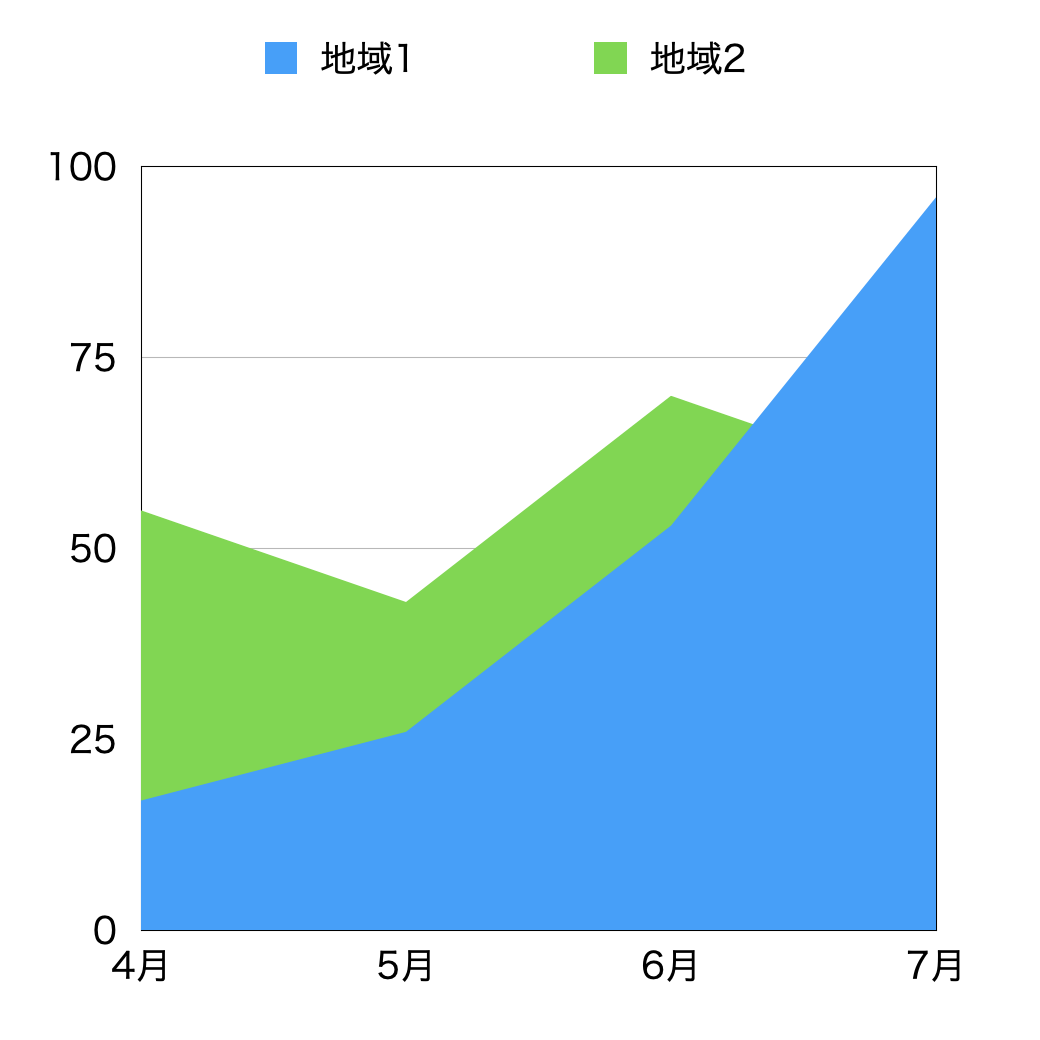
\includegraphics[width=0.5\linewidth]{fig/chart1.png}
  \caption{製品Aの地域別販売状況}
  \label{fig:chart1}
\end{figure}

\section{図の参照}

挿入した図に関係する説明を本文に加える。
その際は本文に図番号を挿入し、どの図に対する説明かがわかるようにする。
例えば「\figref{fig:chart1}に地域1と地域2における製品Aの販売状況の推移を示す。地域1の販売は・・・」
のようにその図やグラフが何を表すか・注目をしてほしい点について説明する。
\textcolor{red}{本文で言及をしない図は挿入しない。}

図番号はWordや\LaTeX にある図番号管理機能を利用して入力する。
図番号を本文中に直接記入をしていると、執筆の過程で図の数や掲載順が変わった際に大量の修正が必要になる。


\section{図の枠線}

図の境界が曖昧なものは\figref{fig:chart2}のように枠線で囲ってもよい。
なお、電子情報分野における国内外の著名な学術雑誌では図を枠線で囲っていない。
この辺りも教員の指導に従ってほしい。

\begin{figure}[H]
  \centering
  \fbox{
    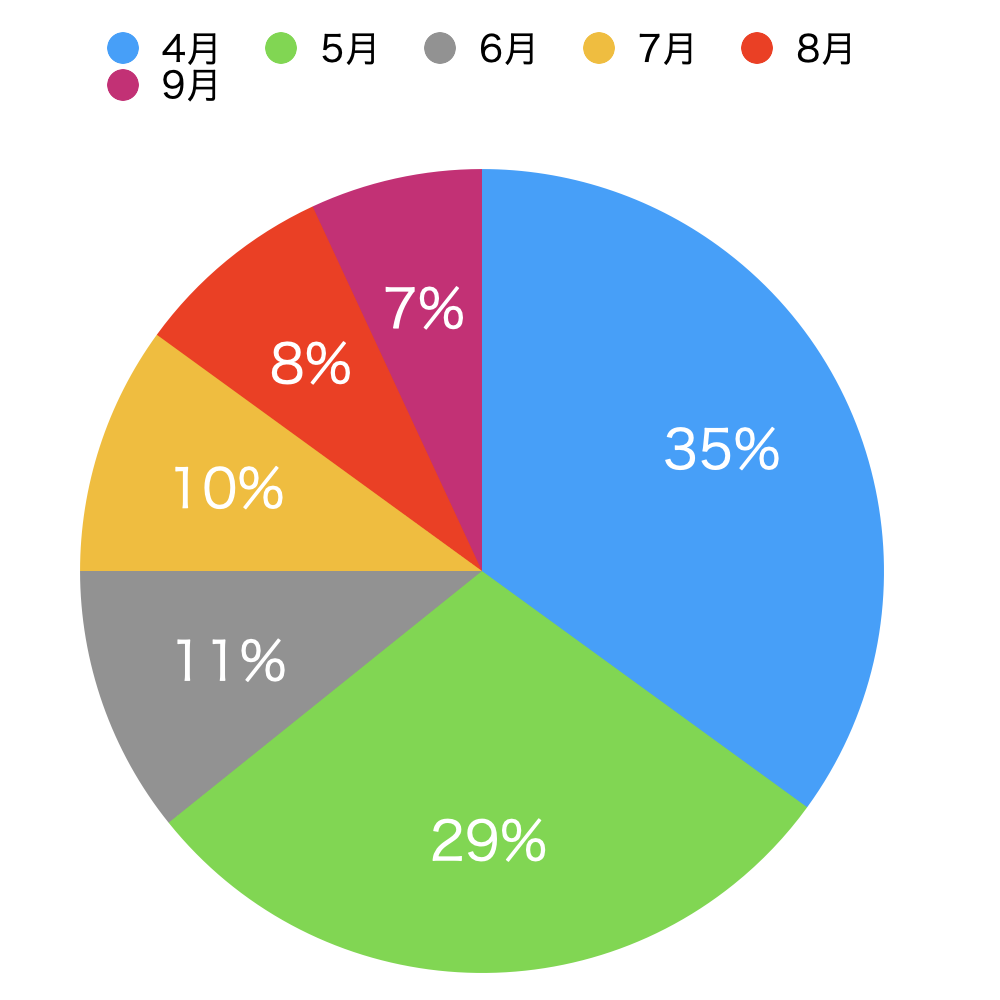
\includegraphics[width=.5\linewidth]{./fig/chart2.png}
  }
  \caption{製品Bの月別売上比率}
  \label{fig:chart2}
\end{figure}

\begin{figure}[H]
  \centering
  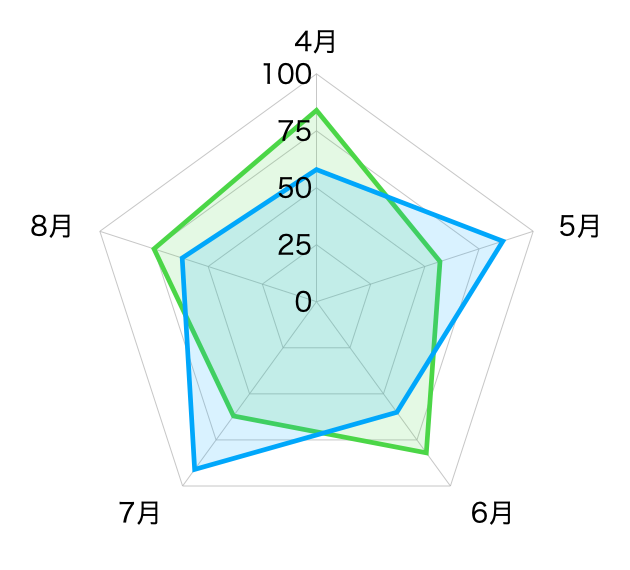
\includegraphics[width=.4\linewidth]{./fig/chart3.png}
  \caption{レーダーチャートの例}
  \label{fig:chart3}
\end{figure}

%%%%%%%%%%%%%%%%%%%%%%%%%%%%%%%%%%%%%%%%%%%%%%%%%%%%%%%%%%%%%%%%%%%%%%%
\begin{comment}
  \begin{textblock}{6.5}(1, 18)
    \noindent
    【16,18】図番号は章ごとの通し番号で抜けがない
  \end{textblock}
  
  \begin{textblock}{7}(13, 22)
    ←本文で説明がない図は載せない
  \end{textblock}
\end{comment}
%%%%%%%%%%%%%%%%%%%%%%%%%%%%%%%%%%%%%%%%%%%%%%%%%%%%%%%%%%%%%%%%%%%%%%%